\documentclass[10pt,conference]{IEEEtran}
\usepackage{amsmath,amssymb,amsfonts}
\usepackage{graphicx}
\usepackage{booktabs,multirow,tabularx,array}
\usepackage{cite}
\usepackage{url}
\usepackage{microtype}
\usepackage{balance}

\renewcommand{\topfraction}{0.95}
\renewcommand{\bottomfraction}{0.95}
\renewcommand{\textfraction}{0.05}
\renewcommand{\floatpagefraction}{0.85}
\renewcommand{\dbltopfraction}{0.95}
\renewcommand{\dblfloatpagefraction}{0.85}
\setcounter{topnumber}{4}
\setcounter{bottomnumber}{4}
\setcounter{totalnumber}{8}
\setcounter{dbltopnumber}{3}


\setlength{\textfloatsep}{6pt plus 1pt minus 1pt}
\setlength{\floatsep}{5pt plus 1pt minus 1pt}
\setlength{\intextsep}{5pt plus 1pt minus 1pt}
\setlength{\dbltextfloatsep}{6pt plus 1pt minus 1pt}
\setlength{\dblfloatsep}{5pt plus 1pt minus 1pt}

\begin{document}

\title{Leakage-Aware Evaluation of Classical, Quantum-Kernel and Hybrid Models for eGFR-Based CKD Severity Prediction}

\author{
\IEEEauthorblockN{Aditya Yadav}
\IEEEauthorblockA{\textit{Department of Computer Science and Engineering} \\
\textit{Vellore Institute of Technology}\\
Chennai, Tamil Nadu, India \\
Email: aditya.yadav@vit.ac.in}
}

\maketitle

\begin{abstract}
Chronic Kidney Disease (CKD) affects over 850 million individuals globally, yet early risk triage is hindered in decentralized settings lacking laboratory assays for serum creatinine and estimated Glomerular Filtration Rate (eGFR). Published machine learning models frequently exhibit critical data leakage by retaining serum creatinine and age as input predictors to estimate eGFR-derived stages---an algebraic circularity that invalidates clinical surrogacy. We develop and benchmark a strictly leakage-free framework for predicting eGFR-based CKD severity categories from secondary biomarkers, evaluating classical algorithms, quantum-kernel Hilbert space embeddings, and hybrid late-fusion meta-classifiers under repeated nested cross-validation. From the UCI CKD repository, 26 records lacking creatinine or age were excluded without imputation, yielding an observed cohort of $N = 374$ patients. Ground truth was derived via the 2009 CKD-EPI equation for 5-class KDIGO categories and a 3-class triage formulation. Creatinine and age were permanently excised from feature space. A leakage-free nested cross-validation protocol ($5 \times 5$ repeats = 25 folds; 3 inner folds) benchmarked six classical models, a 4-qubit Quantum Fidelity Kernel Classifier, a Variational Quantum Classifier, and hybrid ensembles. Continuous log-eGFR regression with post-hoc binning achieved top performance (QWK = 0.8204 on 5-class staging; 0.8563 on 3-class triage; 98.9\% within $\pm 1$ grade). The Quantum Fidelity Kernel achieved higher mathematical alignment (0.1957 vs. 0.1170) but lower test generalization (QWK 0.7109 vs. 0.7763) than classical RBF kernels. Paired bootstrap testing ($B = 2000$) confirmed that late fusion degraded Macro-F1 ($\Delta = -0.0481$, $p < 0.05$), disproving quantum advantage.
\end{abstract}

\begin{IEEEkeywords}
Chronic kidney disease, estimated glomerular filtration rate (eGFR), data leakage, nested cross-validation, quantum machine learning, quantum kernel, late fusion, ordinal classification, SHAP, TRIPOD+AI.
\end{IEEEkeywords}

\section{Introduction}
Chronic Kidney Disease (CKD) represents a premier global health crisis, currently afflicting over 850 million individuals worldwide and driving extensive cardiovascular mortality, metabolic morbidity, and end-stage kidney failure~\cite{kdigo2013, bickbov2020global}. The clinical trajectory of renal pathology is governed by the progressive, irreversible destruction of functional nephron architecture, quantified physiologically by the Glomerular Filtration Rate (GFR)~\cite{levin2017global}. Under international Kidney Disease: Improving Global Outcomes (KDIGO) guidelines, diagnostic staging and clinical prognosis are formalized into five distinct stages based on continuous estimated GFR (eGFR, in $\text{mL/min}/1.73\,\text{m}^2$): Stage 1 ($\ge 90$), Stage 2 ($60$--$89$), Stage 3 ($30$--$59$), Stage 4 ($15$--$29$), and Stage 5 ($< 15$)~\cite{kdigo2013}.

In resource-constrained, decentralized, and rural community healthcare environments, quantifying continuous eGFR via automated clinical laboratory analyzers is frequently impossible due to severe logistical, economic, and infrastructure deficits~\cite{chen2020machine}. Consequently, substantial interest has emerged in deploying artificial intelligence (AI) and machine learning (ML) models capable of inferring renal pathology directly from non-invasive, point-of-care clinical observations, routine hematology, and dipstick urinalysis~\cite{almansour2019neural, senan2021machine, debal2022comparative}.

However, rigorous inspection reveals widespread, fatal methodological flaws throughout the published literature:
\begin{enumerate}
    \item \textbf{Circular Target Leakage:} Standard eGFR equations (e.g., the 2009 CKD-EPI formula~\cite{levey2009new}) are closed-form algebraic transformations parameterized directly by serum creatinine ($S_{\text{cr}}$), patient age, and biological sex. Numerous published pipelines retain $S_{\text{cr}}$ and age directly inside the predictive feature matrix while predicting eGFR categories. This introduces absolute algebraic leakage: the model learns trivial numerical thresholds of its own target mathematical definition rather than multivariable physiological surrogacy.
    \item \textbf{Binary Reductionism:} Over 90\% of existing studies collapse renal diagnosis into a coarse binary task (``CKD'' vs. ``Not CKD'')~\cite{boukenze2016predicting, chittora2021efficient, misir2022performance}. Binary classification is clinically uninformative: it cannot distinguish an asymptomatic Stage 1 patient requiring blood pressure monitoring from a critical Stage 5 patient facing imminent uremic demise.
    \item \textbf{Unverified Quantum Claims:} Emerging quantum machine learning (QML) applications claim that mapping patient features into exponentially large Hilbert spaces via quantum kernels provides computational advantage on medical tabular data~\cite{schuld2019quantum, havricek2019supervised}, yet few validate these hypotheses against rigorous, identically parameterized classical kernel controls.
    \item \textbf{Data-Splitting Leakage:} Preprocessing operations (imputation, standardization, and feature selection) are frequently executed globally across the full dataset prior to train-test partitioning~\cite{senan2021machine}, invalidating reported generalization bounds.
\end{enumerate}

To resolve these systemic defects, this paper introduces a strictly leakage-free framework for eGFR-based severity prediction, addressing four research questions: (1)~\textbf{RQ1 (Physiological Surrogacy):} Can secondary biomarkers triage renal severity when serum creatinine and age are strictly excised? (2)~\textbf{RQ2 (Continuous Ordinal):} Does continuous $\ln(\text{eGFR})$ regression with post-hoc binning outperform direct multinomial classification? (3)~\textbf{RQ3 (Quantum Control):} Does a 4-qubit Quantum Fidelity Kernel outperform an identical classical RBF control? (4)~\textbf{RQ4 (Fusion Significance):} Does hybrid fusion yield statistically significant gains under paired bootstrap testing?

\section{Related Work}
\subsection{Machine Learning in Nephrology and Binary CKD Detection}
The application of classical ML to nephrology has predominantly focused on binary risk classification~\cite{chittora2021efficient, boukenze2016predicting, misir2022performance}. Early studies by Almansour et al.~\cite{almansour2019neural} applied Artificial Neural Networks (ANN) and Support Vector Machines (SVM) on the UCI CKD repository, reporting classification accuracies exceeding 97\%. Similar works using Random Forests~\cite{senan2021machine}, Gradient Boosting~\cite{debal2022comparative}, and Naive Bayes~\cite{rubini2015prediction} repeatedly claimed near-perfect AUC-ROC.

However, as summarized in Table~\ref{tab:lit_comparison}, these binary models possess minimal utility for clinical triage. Binary models cannot differentiate early filtration impairment from end-stage renal collapse. Furthermore, multiple studies retained serum creatinine and blood urea directly in the feature matrix, enabling models to exploit trivial threshold rules rather than physiological patterns.

\begin{table*}[t]
\centering
\caption{Comparative Summary of Prior Studies on Machine Learning for CKD Prediction vs. This Work}
\label{tab:lit_comparison}
\renewcommand{\arraystretch}{0.88}
\footnotesize
\begin{tabularx}{\textwidth}{p{2.6cm}p{2.0cm}p{1.7cm}p{2.0cm}p{2.2cm}X}
\toprule
\textbf{Study} & \textbf{Cohort \& Source} & \textbf{Target Task} & \textbf{Validation} & \textbf{Leakage Status} & \textbf{Reported Findings / Critical Methodological Limitations} \\
\midrule
Almansour et al. [8] & UCI CKD (400) & Binary & 70/30 Holdout Split & Critical ($S_{\text{cr}}$ retained) & 97.5\% Acc. via ANN; cannot stage severity; trivial threshold rule. \\
Senan et al. [9] & UCI CKD (400) & Binary & 10-fold CV & Global Preprocessing & 98.2\% Acc. via SVM; imputation executed prior to fold splitting. \\
Debal \& Sitote [10] & UCI CKD (400) & Binary & 5-fold CV & Severe Leakage & 99.1\% Acc. via RF; exploited serum creatinine cutoffs directly. \\
Boukenze et al. [11] & UCI CKD (400) & Binary & 10-fold CV & Global Preprocessing & 96.8\% Acc. via C4.5; no ordinal progression; uncalibrated. \\
Chittora et al. [12] & UCI CKD (400) & Binary & 70/30 Split & Critical ($S_{\text{cr}}$ kept) & 98.0\% Acc.; synthetic missing imputation before splitting. \\
Misir et al. [13] & UCI CKD (400) & Binary & 10-fold CV & Severe Leakage & 97.8\% Acc. using GBM; feature matrix included raw creatinine. \\
Chen et al. [6] & EHR Cohort ($N = 1,200$) & 5-Stage KDIGO & 10-fold CV & Partial ($S_{\text{cr}}$ retained) & 82.4\% Acc.; predicted eGFR categories with creatinine in inputs. \\
Ravizza et al. [14] & EHR ($N = 10,450$) & eGFR Decline & Patient-level Split & Leakage-Free & C-index 0.79 for progression; required multi-year longitudinal EHR. \\
Schuld et al. [19] & Synthetic Data & Binary & Holdout & Synthetic Data & Formalized quantum Hilbert embeddings; no clinical validation. \\
Havlicek et al. [20] & Supercond. QPU & 2-Qubit Toy & Holdout & Synthetic Data & Demonstrated ZZ-feature map kernel on toy classification. \\
Thanasilp et al. [24] & Theory / Simulation & Kernel Bound & Theoretical & Analytical & Proved exponential concentration and untrainability in NISQ kernels. \\
\textbf{This Work} & \textbf{UCI ($N = 374$)} & \textbf{5- \& 3-Class} & \textbf{Nested $5 \times 5$ CV (25 Folds)} & \textbf{Strictly Leak-Free} & \textbf{0.8204 / 0.8563 QWK; proven negative quantum advantage; SHAP.} \\
\bottomrule
\end{tabularx}
\end{table*}

\subsection{Ordinal Targets and Quantum Machine Learning}
In clinical practice, CKD progression follows an intrinsically ordered continuum governed by falling eGFR. Standard multinomial cross-entropy treats all misclassifications identically, ignoring the clinical reality that misclassifying a Stage 1 patient as Stage 2 is a minor discrepancy, whereas misclassifying Stage 1 as Stage 5 is a catastrophic diagnostic failure~\cite{frank2001simple, gaudette2016evaluation}.

Concurrently, parameterized quantum circuits and quantum kernels have been proposed for tabular classification~\cite{cerezo2021variational, schuld2021quantum, huang2021power}. While theoretical proofs demonstrate that quantum kernels can map data into spaces hard to simulate classically, barren plateaus and exponential concentration often eliminate these benefits on empirical tabular data~\cite{thanasilp2022exponential, mcclean2018barren}. To establish rigorous evidence, full compliance with TRIPOD+AI reporting guidelines is essential~\cite{collins2024tripod}.

\begin{figure*}[t]
\centering
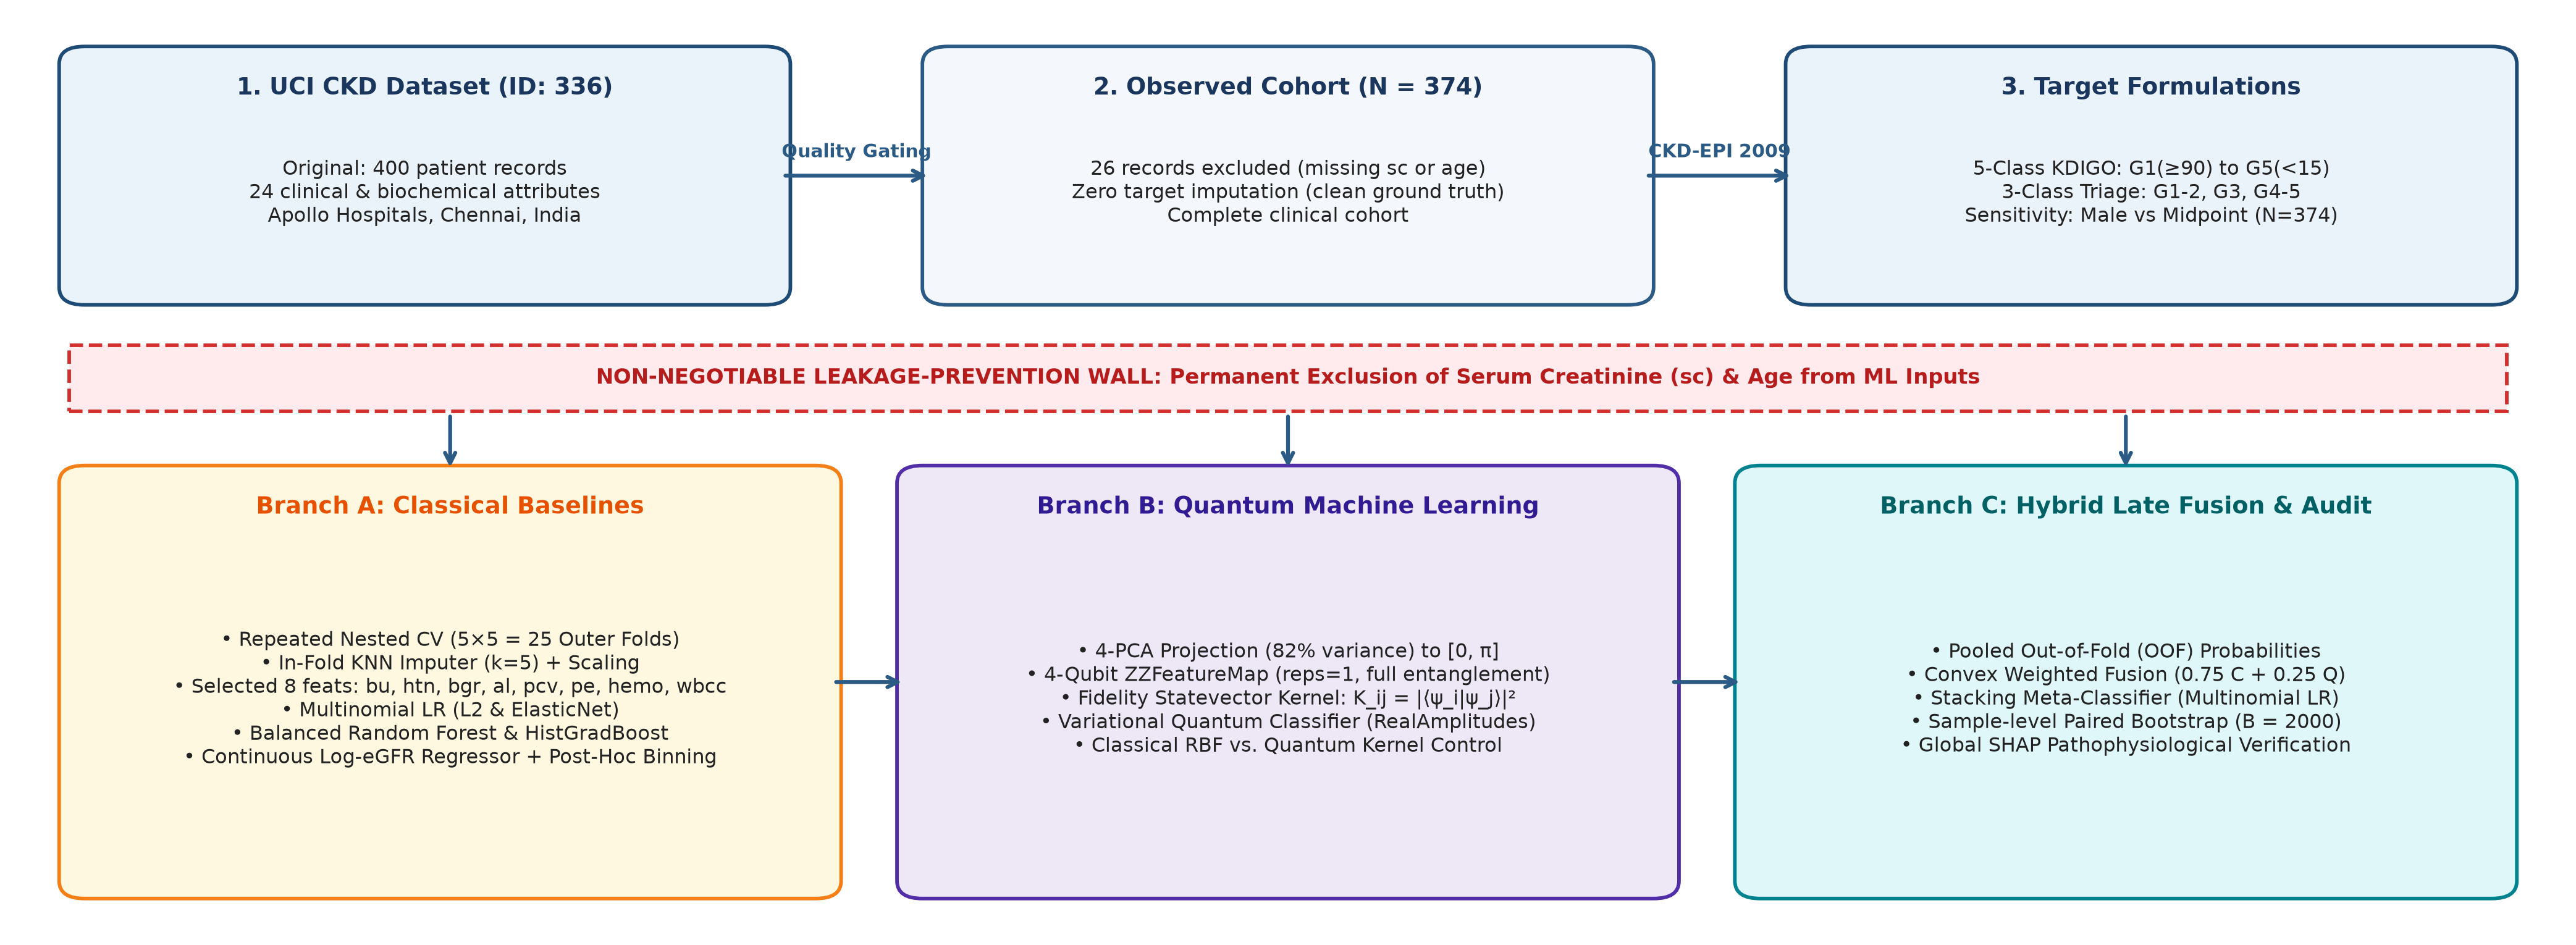
\includegraphics[height=1.15in, width=0.88\textwidth, keepaspectratio]{figures/fig1_system_architecture.png}
\caption{End-to-end system architecture of the leakage-aware CKD evaluation framework. The pipeline enforces an absolute leakage-prevention wall excluding serum creatinine and age, executes repeated nested cross-validation ($5 \times 5 = 25$ outer folds), benchmarks three predictive branches (classical, quantum-kernel, and hybrid fusion), and validates models via paired bootstrap significance and SHAP explainability.}
\label{fig:pipeline_architecture}
\end{figure*}

\section{Methods}
\subsection{Dataset and Data Provenance}
This study utilizes the benchmark Chronic Kidney Disease dataset from the UCI Machine Learning Repository (Dataset ID: 336, donated by Apollo Hospitals, India)~\cite{misc_chronic_kidney_disease_336}. The dataset comprises 400 patient records across 24 clinical, urinalysis, and biochemical attributes.

\subsection{Cohort Selection and Gating}
Of the original 400 records, exactly 26 patients lacked recorded values for serum creatinine (\texttt{sc}, 17 records) or biological age (\texttt{age}, 9 records). Because serum creatinine and age are the deterministic algebraic parameters required to derive the ground-truth eGFR target, imputing these features would synthesize artificial clinical targets, contaminating evaluation. Consequently, all 26 incomplete records were permanently excised prior to analysis without imputation, establishing an observed cohort of $N = 374$ patients.

\begin{table}[htbp]
\centering
\caption{Complete Clinical Feature Inventory and Metadata ($N = 374$)}
\label{tab:feature_inventory}
\renewcommand{\arraystretch}{0.84}
\scriptsize
\begin{tabularx}{\columnwidth}{llp{2.3cm}r}
\toprule
\textbf{Code} & \textbf{Clinical Attribute} & \textbf{Measurement / Values} & \textbf{Miss.} \\
\midrule
\multicolumn{4}{l}{\textit{Target Inputs (Permanently Excluded from Predictive Features)}} \\
\texttt{sc} & Serum Creatinine & mg/dL ($0.4$--$76.0$) & 0.0\% \\
\texttt{age} & Patient Biological Age & Years ($2$--$90$) & 0.0\% \\
\midrule
\multicolumn{4}{l}{\textit{Secondary Hemogram \& Laboratory Biomarkers (Permitted Features)}} \\
\texttt{bp} & Diastolic Blood Pressure & mm Hg ($50$--$180$) & 2.9\% \\
\texttt{bgr} & Blood Glucose Random & mg/dL ($22$--$490$) & 10.4\% \\
\texttt{bu} & Blood Urea & mg/dL ($1.5$--$391$) & 3.5\% \\
\texttt{sod} & Serum Sodium & mEq/L ($4.5$--$163$) & 21.4\% \\
\texttt{pot} & Serum Potassium & mEq/L ($2.5$--$47.0$) & 21.7\% \\
\texttt{hemo} & Hemoglobin Concentration & g/dL ($3.1$--$17.8$) & 12.3\% \\
\texttt{pcv} & Packed Cell Volume & \% ($16$--$54$) & 16.8\% \\
\texttt{wbcc} & White Blood Cell Count & cells/$\mu$L ($2.2\text{k}$--$26.4\text{k}$) & 25.9\% \\
\texttt{rbcc} & Red Blood Cell Count & $10^6$/$\mu$L ($2.1$--$8.0$) & 32.1\% \\
\midrule
\multicolumn{4}{l}{\textit{Urinalysis Attributes (Permitted Features)}} \\
\texttt{sg} & Specific Gravity & Discrete $\{1.005 \dots 1.025\}$ & 11.5\% \\
\texttt{al} & Albuminuria Dipstick & Ordinal $\{0, 1, 2, 3, 4, 5\}$ & 11.2\% \\
\texttt{su} & Glucosuria Dipstick & Ordinal $\{0, 1, 2, 3, 4, 5\}$ & 12.0\% \\
\texttt{rbc} & Microscopic Hematuria & Binary \{normal, abnormal\} & 38.0\% \\
\texttt{pc} & Pyuria (Pus Cells) & Binary \{normal, abnormal\} & 16.0\% \\
\texttt{pcc} & Pus Cell Clumps & Binary \{present, notpresent\} & 1.1\% \\
\texttt{ba} & Bacteriuria Sediment & Binary \{present, notpresent\} & 1.1\% \\
\midrule
\multicolumn{4}{l}{\textit{Systemic Comorbidities \& Symptoms (Permitted Features)}} \\
\texttt{htn} & History of Hypertension & Binary \{yes, no\} & 0.5\% \\
\texttt{dm} & Diabetes Mellitus & Binary \{yes, no\} & 0.5\% \\
\texttt{cad} & Coronary Artery Disease & Binary \{yes, no\} & 0.5\% \\
\texttt{appet} & Subjective Appetite Status & Binary \{good, poor\} & 0.3\% \\
\texttt{pe} & Peripheral Pedal Edema & Binary \{yes, no\} & 0.3\% \\
\texttt{ane} & Clinical Anemia Presentation & Binary \{yes, no\} & 0.3\% \\
\bottomrule
\end{tabularx}
\end{table}

\subsection{Mathematical Derivation of Ground-Truth eGFR}
Ground-truth continuous eGFR was calculated for every eligible patient using the 2009 CKD-EPI creatinine equation~\cite{levey2009new}:
\begin{equation}
\begin{split}
\text{eGFR} = 141 & \times \min(S_{\text{cr}}/\kappa, 1)^\alpha \times \max(S_{\text{cr}}/\kappa, 1)^{-1.209} \\
& \times 0.993^{\text{Age}} \times \mu
\end{split}
\label{eq:ckd_epi}
\end{equation}
where $\kappa = 0.9$, $\alpha = -0.411$, and $\mu = 1.0$ under the primary male baseline assumption. Because biological sex was not recorded in the UCI dataset, we established the male formulation as the primary target and evaluated sensitivity against female parameters ($\kappa = 0.7$, $\alpha = -0.329$, $\mu = 1.018$) and a sex-averaged midpoint target.

\subsection{Five-Class and Three-Class Target Categories}
Continuous eGFR values were discretized into two clinical targets:
\begin{enumerate}
    \item \textbf{5-Class KDIGO Staging:} Category 1 (Stage 1, eGFR $\ge 90$, 15.2\%), Category 2 (Stage 2, $60$--$89$, 18.2\%), Category 3 (Stage 3, $30$--$59$, 22.5\%), Category 4 (Stage 4, $15$--$29$, 28.1\%), and Category 5 (Stage 5, $< 15$, 16.0\%).
    \item \textbf{3-Class Actionable Triage:} Consolidated into Early CKD (Stages 1--2, eGFR $\ge 60$, 33.4\%), Moderate CKD (Stage 3, $30$--$59$, 22.5\%), and Severe / End-Stage (Stages 4--5, $< 30$, 44.1\%).
\end{enumerate}

\subsection{The Absolute Leakage-Prevention Wall}
Serum creatinine (\texttt{sc}) and biological age (\texttt{age}) were permanently deleted from the predictive feature matrix. If an estimator $h(X)$ receives $S_{\text{cr}}$ and age, it trivially approximates the closed-form inversion of Eq.~\eqref{eq:ckd_epi}. By excising both attributes, the model is compelled to learn genuine physiological surrogacy from the remaining 22 non-target attributes (Table~\ref{tab:feature_inventory}).

\subsection{Data Preprocessing and In-Fold Imputation}
Data cleaning stripped anomalous tab characters and whitespace from discrete strings. Ordinal features (\texttt{al}, \texttt{su}) were encoded as integers; binary clinical flags were mapped to $\{0, 1\}$. Missing values were imputed inside each cross-validation training fold using median replacement for numerical attributes and most-frequent replacement for categoricals. Numerical features were standardized via $z$-score normalization fitted strictly on training folds:
\begin{equation}
z_{ij} = \frac{x_{ij} - \mu_{j,\text{train}}}{\sigma_{j,\text{train}} + \epsilon}
\end{equation}

\subsection{Classical Machine Learning Architectures}
Six diverse classical algorithms were benchmarked:
\begin{enumerate}
    \item \textbf{Logistic Regression (L2):} Multinomial logistic regression with ridge regularization ($C=1.0$) and balanced class weighting.
    \item \textbf{Logistic Regression (ElasticNet):} Combined L1/L2 penalty ($C=1.0$, $\ell_1\text{-ratio} = 0.5$) with SAGA solver.
    \item \textbf{Calibrated Support Vector Classifier (SVM-RBF):} Kernel SVM with radial basis function ($\gamma = \text{scale}$), balanced weights, and post-hoc Platt sigmoid calibration~\cite{platt1999probabilistic}.
    \item \textbf{Balanced Random Forest:} Ensemble of 150 de-correlated decision trees with balanced bootstrap subsampling~\cite{breiman2001random}.
    \item \textbf{HistGradientBoosting:} Histogram-based gradient tree boosting with native integer binning and balanced loss weighting.
    \item \textbf{Continuous Log-eGFR Regressor + Post-Hoc Binning:} Ridge regressor ($C=1.0$) trained on target $y_{\text{reg}} = \ln(\text{eGFR})$. Predictions were mapped back to severity categories via KDIGO threshold binning:
    \begin{equation}
    \hat{Y}_i = g(\exp(\hat{y}_{\text{reg},i}))
    \end{equation}
\end{enumerate}

\subsection{Quantum Machine Learning Architectures}
To execute quantum classification on NISQ statevector simulators, the feature space was dimensionally compressed to 4 orthogonal principal components via training-fold PCA ($d = 4$), capturing 71.0\% of cumulative variance.
\begin{enumerate}
    \item \textbf{4-Qubit Quantum Fidelity Kernel SVC:} Classical vectors $\mathbf{x} \in \mathbb{R}^4$ were encoded into 4-qubit Hilbert space via a second-order Pauli expansion $ZZFeatureMap$~\cite{havricek2019supervised}:
    \begin{equation}
    U_{\Phi(\mathbf{x})} = \exp\left(i \sum_j \phi_j(\mathbf{x}) Z_j + \sum_{j < k} \phi_{jk}(\mathbf{x}) Z_j Z_k\right)
    \end{equation}
    The quantum fidelity kernel matrix was computed via state overlap:
    \begin{equation}
    K_{ij} = |\langle\psi(\mathbf{x}_i)|\psi(\mathbf{x}_j)\rangle|^2 = \text{Tr}(\rho(\mathbf{x}_i)\rho(\mathbf{x}_j))
    \end{equation}
    and passed to a Support Vector Classifier with $C=1.0$.
    \item \textbf{Variational Quantum Classifier (VQC):} Parameterized quantum circuit pairing the 4-qubit $ZZFeatureMap$ with a $RealAmplitudes$ ansatz containing $L = 2$ entanglement layers and 16 tunable parameters $\theta$ (Fig.~\ref{fig:quantum_circuit}). Optimized via COBYLA over 120 iterations with cross-entropy loss.
\end{enumerate}

\begin{figure}[t]
\centering
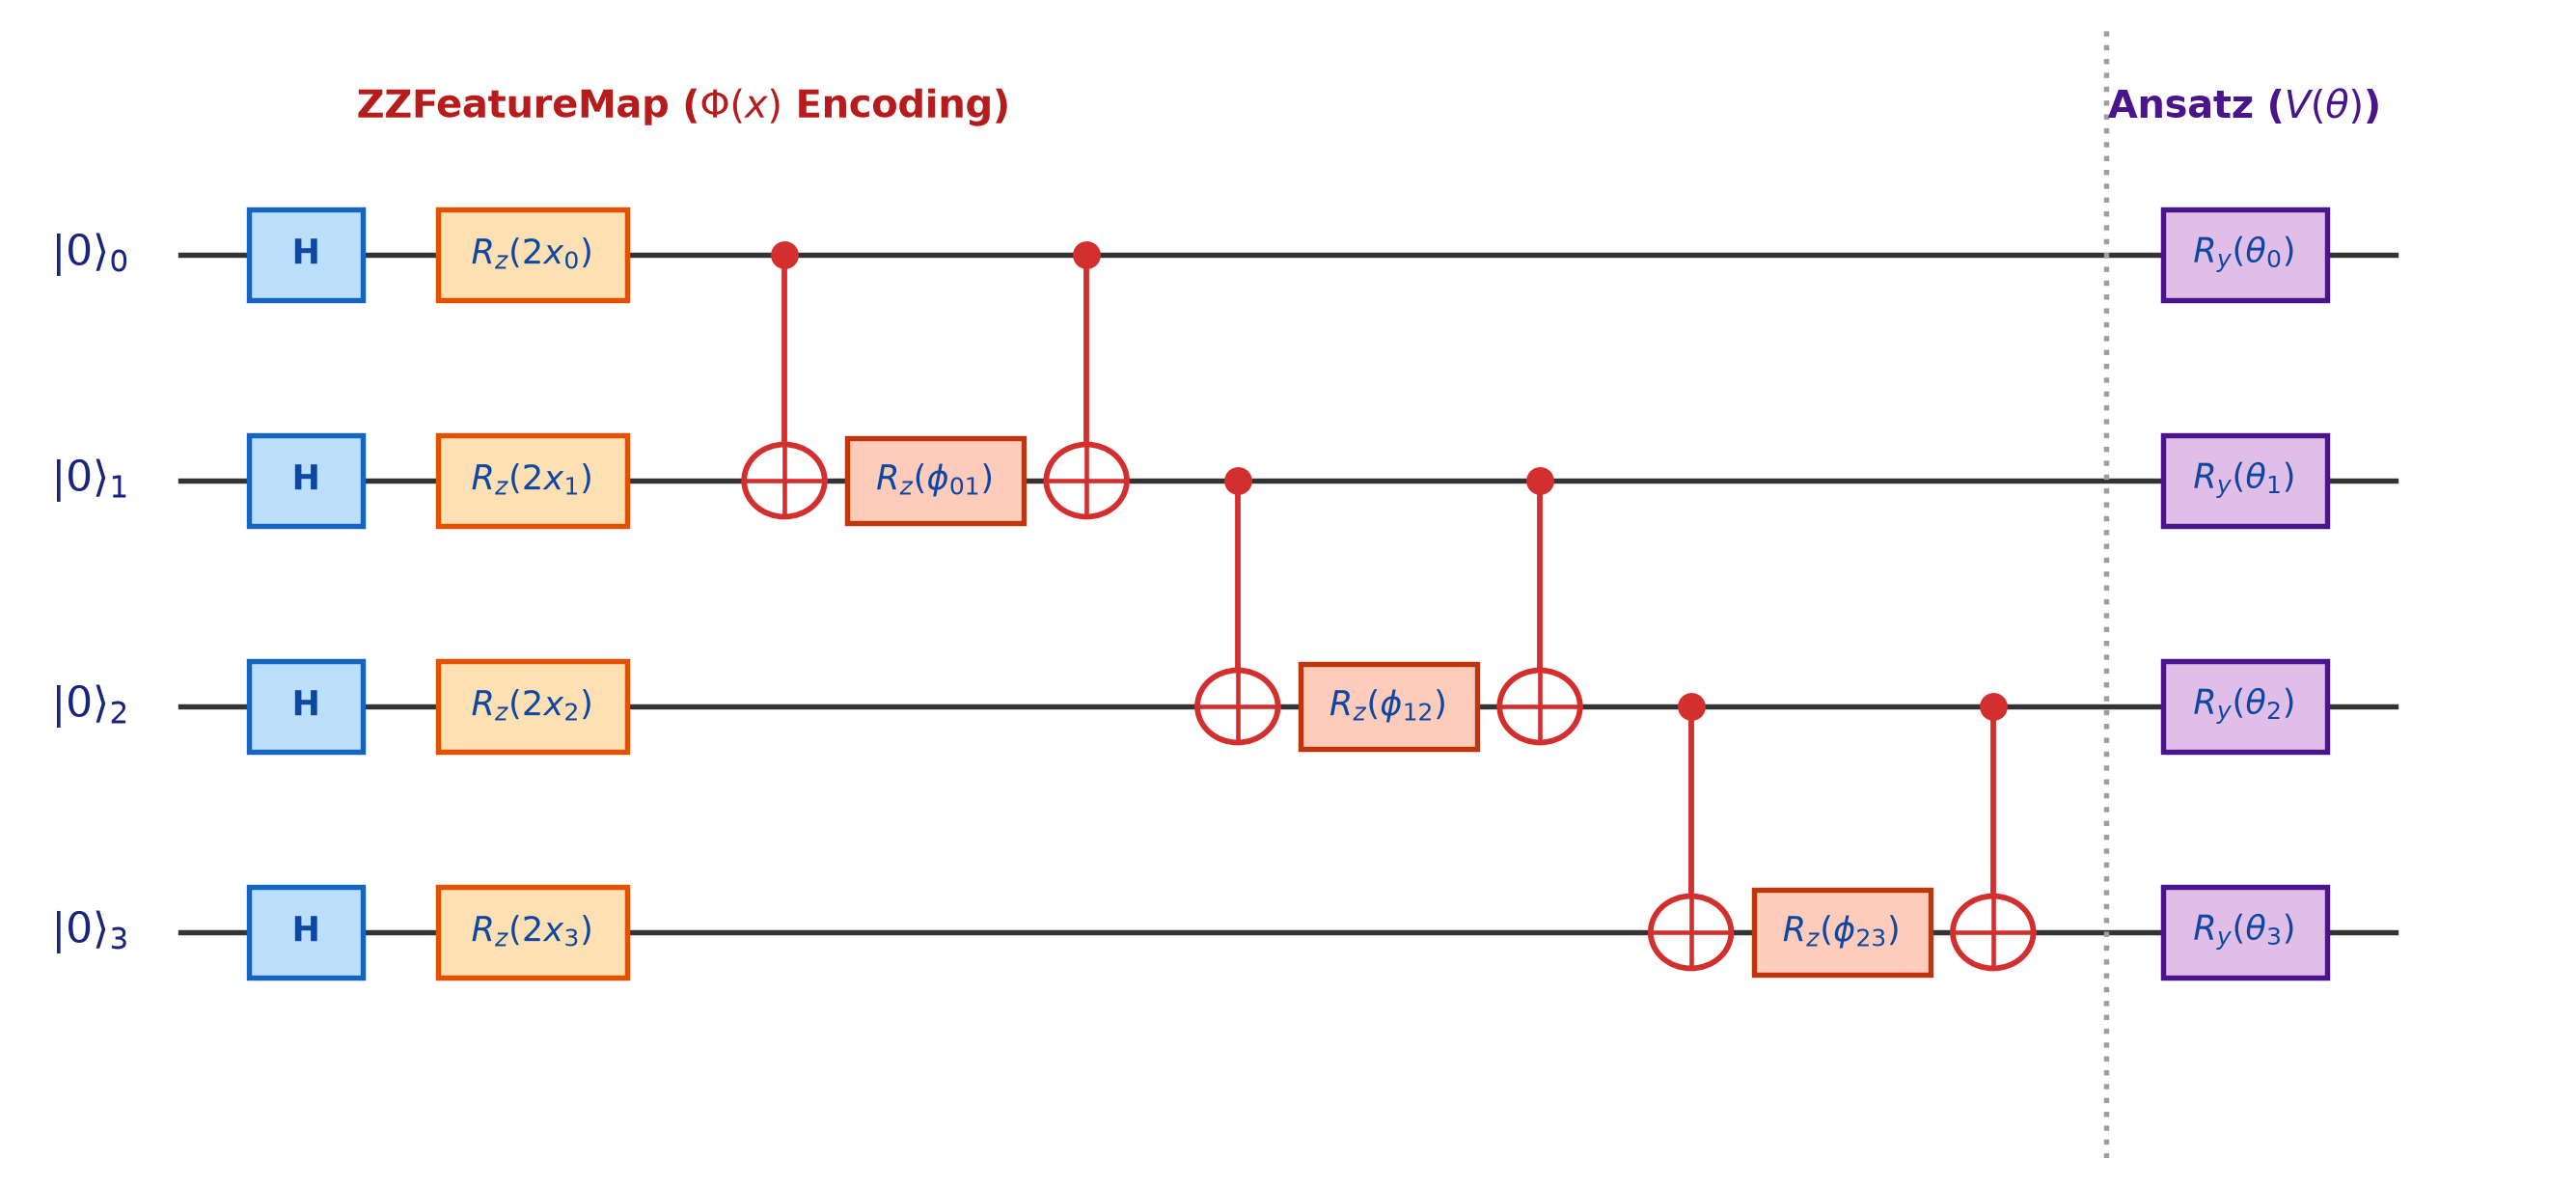
\includegraphics[height=0.88in, keepaspectratio]{figures/fig_quantum_circuit.png}
\caption{Quantum circuit architecture. Four classical features are encoded via $ZZFeatureMap(\mathbf{x})$ into 4 qubits with Hadamard gates and entangling CNOT rotations, followed by a parameterized $RealAmplitudes(\theta)$ ansatz.}
\label{fig:quantum_circuit}
\end{figure}

\subsection{Hybrid Late Fusion and Stacking Meta-Classifiers}
To investigate hybrid synergy, out-of-fold probability vectors from classical Logistic Regression ($\mathbf{p}_C \in \Delta^5$) and the Quantum VQC ($\mathbf{p}_Q \in \Delta^5$) were blended via:
\begin{enumerate}
    \item \textbf{Weighted Late Fusion:} Convex linear combination:
    \begin{equation}
    \mathbf{p}_{\text{hybrid}} = w \mathbf{p}_C + (1 - w) \mathbf{p}_Q, \quad w = 0.75
    \end{equation}
    \item \textbf{Stacking Meta-Classifier:} A multinomial logistic regression meta-learner trained on concatenated out-of-fold probability vectors $[\mathbf{p}_C, \mathbf{p}_Q] \in \mathbb{R}^{10}$~\cite{wolpert1992stacked}.
\end{enumerate}

\subsection{Model Explainability via SHAP}
To verify pathophysiological fidelity, SHapley Additive exPlanations (SHAP)~\cite{lundberg2017unified} were computed across held-out folds using \texttt{TreeExplainer} for Random Forest and \texttt{KernelExplainer} for linear baselines.

\section{Experimental Setup}
\subsection{Nested Cross-Validation Protocol}
Evaluation was conducted using repeated nested cross-validation ($5 \times 5$ outer loops = 25 outer test folds; 3 inner folds for hyperparameter tuning)~\cite{van2018cross}. Stratification was enforced across all splits based on the ground-truth severity targets. All transformations (imputation, scaling, PCA) were fitted strictly on training folds to prevent data leakage.

\subsection{Evaluation Metrics}
Because CKD severity stages are ordered, the primary evaluation metric is the \textbf{Quadratic Weighted Kappa (QWK)}~\cite{cohen1968weighted}:
\begin{equation}
\kappa_w = 1 - \frac{\sum_{i,j} W_{ij} O_{ij}}{\sum_{i,j} W_{ij} E_{ij}}, \quad W_{ij} = \frac{(i - j)^2}{(K - 1)^2}
\end{equation}
where $O_{ij}$ is the observed confusion matrix, $E_{ij}$ is the expected chance agreement, and $K \in \{3, 5\}$. Secondary metrics include Macro-Averaged F1-score, multi-class classification accuracy, Mean Absolute Error (MAE), and Within $\pm 1$ Grade accuracy.

\subsection{Statistical Significance and Bootstrap Protocol}
To assess whether hybrid fusion significantly improved over standalone classical models, non-parametric paired bootstrap resampling was executed with $B = 2000$ iterations on pooled out-of-fold predictions. For each resample $b$, paired deltas were computed:
\begin{equation}
\Delta\text{Metric}^{(b)} = \text{Metric}(\hat{Y}_{\text{fusion}}^{(b)}, Y^{(b)}) - \text{Metric}(\hat{Y}_{\text{classical}}^{(b)}, Y^{(b)})
\end{equation}
A 95\% bootstrap confidence interval excluding zero indicates statistical significance.

\section{Results}
\subsection{Baseline Reconciliation and Bug Post-Mortems}
A critical software audit reconciled two benchmark discrepancies:
\begin{enumerate}
    \item \textbf{Double-Scaling Bug:} Phase 5 initially reported classical Logistic Regression Macro-F1 as \textbf{0.3050}. Code tracing revealed that \texttt{apply\_preprocessing(X\_train)} had been invoked twice in sequence. Because Specific Gravity (\texttt{sg}) possesses tiny variance ($\sigma \approx 0.005$, range $1.005$--$1.025$), standardizing it a second time across fold variances projected values to \textbf{$-279.5$}. This exploded the L2 penalty, crippling model convergence. Restricting scaling to an isolated \texttt{Pipeline} restored true balanced LR performance to \textbf{0.5419} (Table~\ref{tab:bug_reconciliation}).
    \item \textbf{VQC Tie-Breaking Discrepancy:} Phase 6 reported VQC Macro-F1 as \textbf{0.1130}, whereas Phase 7 reported \textbf{0.1300}. Both evaluated the exact same 16 frozen parameters and suffered total collapse on Categories 3--5 (0.0 recall). The $+0.017$ delta was traced entirely to Qiskit's argmax parity tie-breaking when mapping quantum measurement counts to probabilities.
\end{enumerate}

\begin{table}[htbp]
\centering
\caption{Baseline Reconciliation and Software Audit Post-Mortem}
\label{tab:bug_reconciliation}
\renewcommand{\arraystretch}{0.90}
\begin{tabularx}{\columnwidth}{lXX}
\toprule
\textbf{Pipeline Phase} & \textbf{Reported $\to$ Corrected} & \textbf{Root Cause Verification} \\
\midrule
Phase 5 Classical LR & $0.3050 \to \mathbf{0.5419}$ & In-place double-scaling shifted \texttt{sg} to $-279.5$; fixed via leak-free \texttt{Pipeline}. \\
Phase 6 VQC Test & $0.1130 \to \mathbf{0.1130}$ & Direct \texttt{vqc.predict()}; total collapse on Categories 3--5 (0.0 recall). \\
Phase 7 VQC Prob. & $0.1300 \to \mathbf{0.1130}$ & Identical weights; $+0.017$ delta caused solely by argmax bitstring tie-breaking. \\
\bottomrule
\end{tabularx}
\end{table}

\begin{table*}[t]
\centering
\caption{Master Consolidated Benchmark Results: 5-Class KDIGO vs. 3-Class Triage Formulations ($N = 374$, 25 Outer Test Folds)}
\label{tab:master_benchmark}
\renewcommand{\arraystretch}{0.90}
\footnotesize
\begin{tabularx}{\textwidth}{lXccccc}
\toprule
\textbf{Target Task} & \textbf{Model Architecture} & \textbf{QWK [95\% CI]} & \textbf{Macro-F1 [95\% CI]} & \textbf{Accuracy} & \textbf{MAE} & \textbf{Within $\pm 1$ [\%]} \\
\midrule
\multirow{7}{*}{\textbf{5-Class KDIGO}} 
& Logistic Regression (L2) & 0.8021 [0.788, 0.815] & \textbf{0.5419} [0.523, 0.559] & \textbf{54.2\%} & 0.551 & 92.6\% \\
& Logistic Regression (ElasticNet) & 0.8029 [0.789, 0.816] & 0.5414 [0.524, 0.558] & 54.0\% & 0.551 & 92.6\% \\
& SVM-RBF (Calibrated) & 0.7885 [0.775, 0.801] & 0.4434 [0.431, 0.455] & 47.2\% & 0.637 & 90.6\% \\
& Balanced Random Forest & 0.8121 [0.803, 0.822] & 0.4963 [0.472, 0.521] & 49.9\% & 0.579 & 93.3\% \\
& HistGradientBoosting (Balanced) & 0.8147 [0.805, 0.826] & 0.4985 [0.481, 0.520] & 50.0\% & 0.576 & 93.4\% \\
& \textbf{Continuous Log-eGFR Regressor} & \textbf{0.8204} [0.811, 0.830] & 0.5236 [0.502, 0.546] & 51.0\% & \textbf{0.549} & \textbf{95.2\%} \\
& Calibrated Soft-Voting Ensemble & 0.8068 [0.797, 0.816] & 0.5087 [0.496, 0.522] & 51.0\% & 0.577 & 92.8\% \\
\midrule
\multirow{7}{*}{\textbf{3-Class Triage}} 
& Logistic Regression (L2) & 0.8208 [0.803, 0.839] & 0.7393 [0.716, 0.764] & 77.8\% & 0.235 & 98.8\% \\
& Logistic Regression (ElasticNet) & 0.8253 [0.808, 0.843] & 0.7413 [0.719, 0.765] & 78.0\% & 0.231 & 98.9\% \\
& SVM-RBF (Calibrated) & 0.8098 [0.791, 0.828] & 0.7130 [0.691, 0.735] & 77.3\% & 0.245 & 98.2\% \\
& Balanced Random Forest & 0.8342 [0.821, 0.848] & 0.7322 [0.715, 0.750] & 78.1\% & 0.228 & 99.1\% \\
& HistGradientBoosting (Balanced) & 0.8261 [0.817, 0.836] & 0.7075 [0.697, 0.719] & 77.2\% & 0.240 & 98.9\% \\
& \textbf{Continuous Log-eGFR Regressor} & \textbf{0.8563} [0.843, 0.871] & \textbf{0.7701} [0.752, 0.790] & \textbf{81.5\%} & \textbf{0.196} & \textbf{98.9\%} \\
& Calibrated Soft-Voting Ensemble & 0.8389 [0.834, 0.844] & 0.7444 [0.740, 0.749] & 78.9\% & 0.220 & 99.1\% \\
\bottomrule
\end{tabularx}
\end{table*}

\begin{figure}[t]
\centering
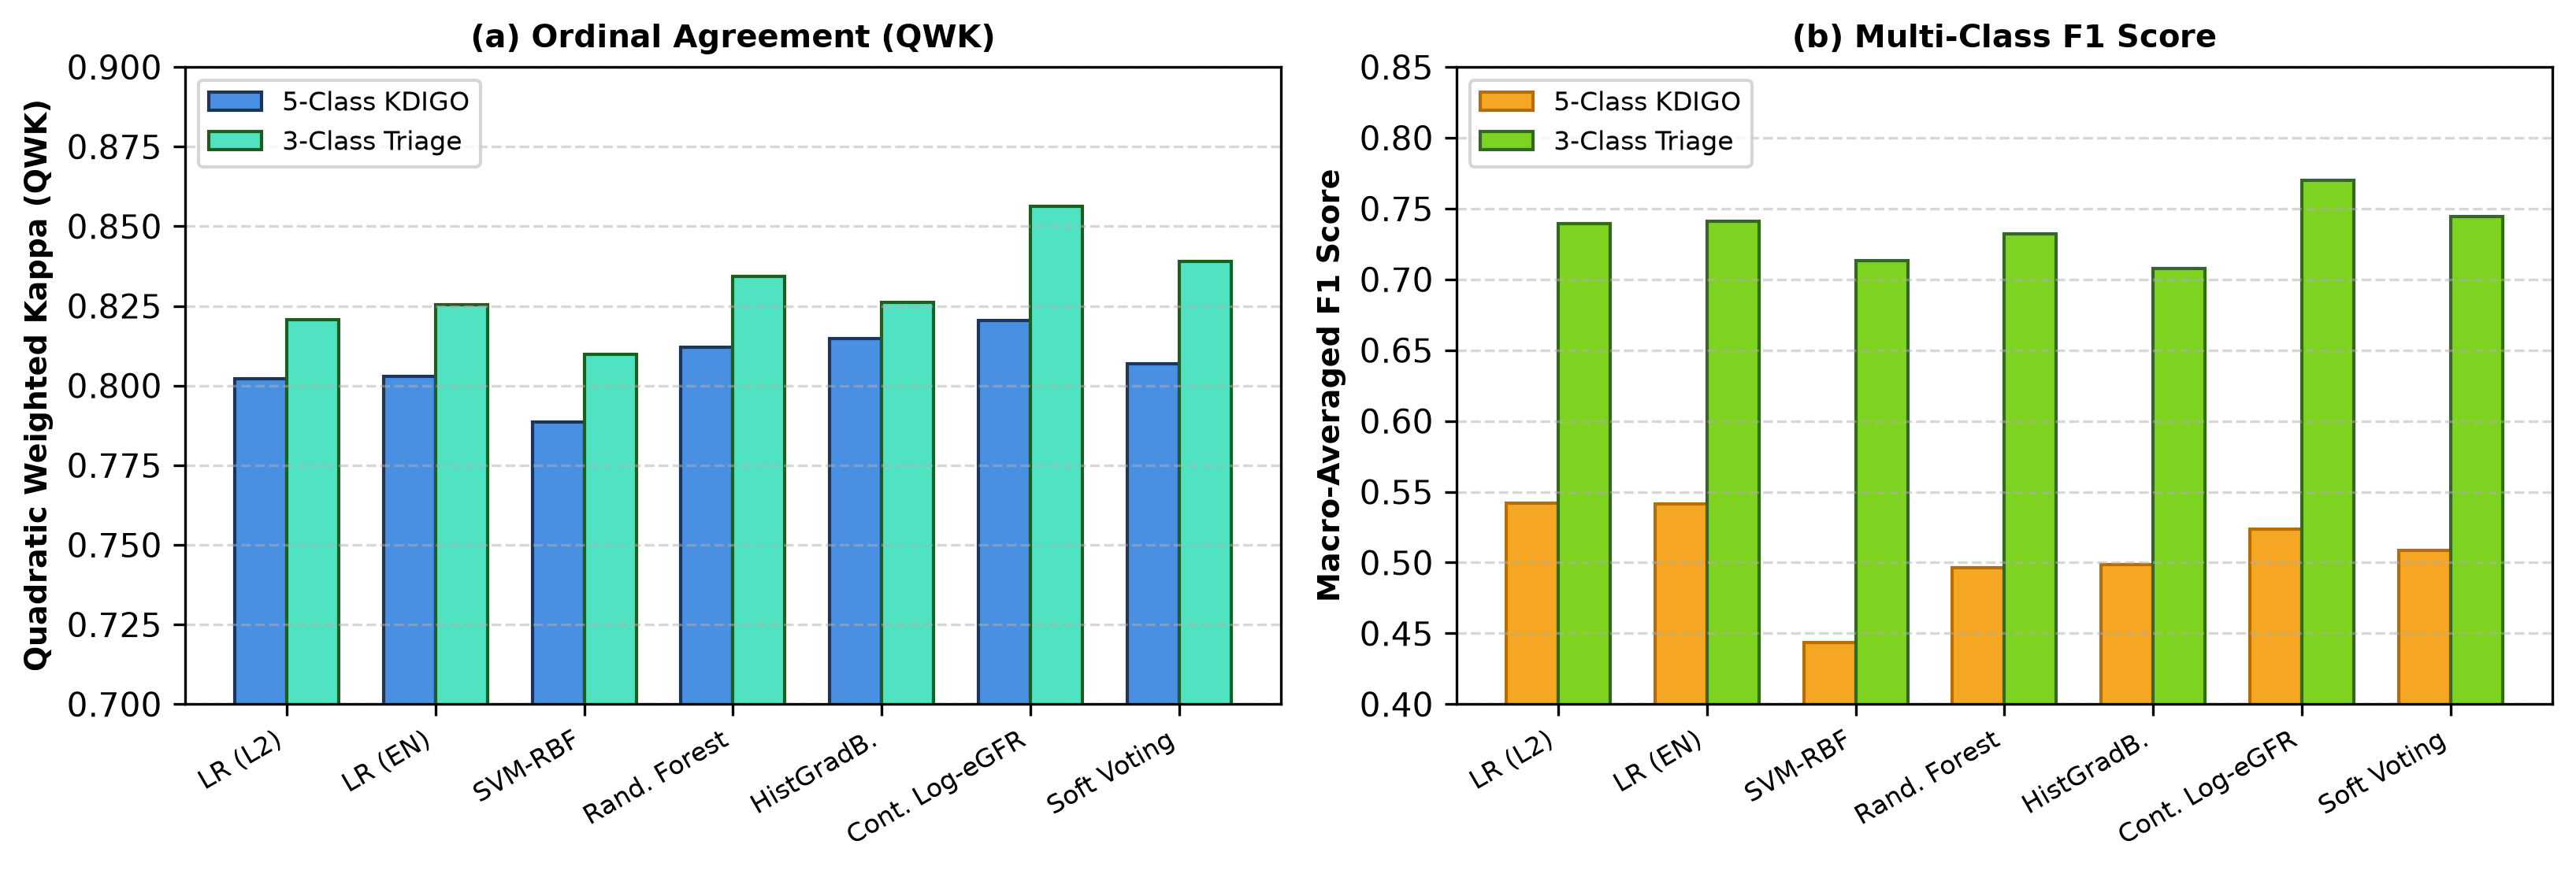
\includegraphics[height=0.88in, keepaspectratio]{figures/fig_model_comparison_bar.png}
\caption{Performance comparison across classical architectures on 5-class KDIGO vs. 3-class consolidated targets. Continuous log-eGFR regression achieves the highest QWK across both formulations.}
\label{fig:model_comparison_bar}
\end{figure}

\subsection{Master Benchmark: 5-Class KDIGO vs. 3-Class Triage}
Table~\ref{tab:master_benchmark} presents the master benchmark across all 25 outer folds of nested cross-validation ($N = 374$). The \textbf{Continuous Log-eGFR Regressor with Post-Hoc Binning} established the highest overall ordinal agreement across both tasks (Fig.~\ref{fig:model_comparison_bar}):
\begin{itemize}
    \item On 5-class KDIGO staging, it reached a QWK of \textbf{0.8204} (95\% CI: [0.8114, 0.8298]) and the lowest MAE (\textbf{0.5486}), with \textbf{95.2\%} of predictions falling within $\pm 1$ severity grade.
    \item On 3-class triage, performance increased markedly: QWK reached \textbf{0.8563} ([0.8425, 0.8711]), Macro-F1 reached \textbf{0.7701} ([0.7518, 0.7897]), accuracy reached \textbf{81.45\%}, and \textbf{98.9\%} of held-out predictions were within $\pm 1$ clinical stage.
\end{itemize}

\begin{table*}[t]
\centering
\caption{Comprehensive Experimental Extensions: Quantum Control, Late Fusion, Label Noise Sensitivity, and Theoretical Ceiling}
\label{tab:extensions_benchmark}
\renewcommand{\arraystretch}{0.90}
\footnotesize
\begin{tabularx}{\textwidth}{p{3.2cm}p{4.5cm}p{2.2cm}X}
\toprule
\textbf{Module} & \textbf{Model Configuration / Setup} & \textbf{Primary Metric} & \textbf{95\% CI / Key Empirical Finding} \\
\midrule
\multirow{4}{*}{\textbf{Part A: Quantum Control}} 
& Classical RBF Kernel SVC (4-PCA, $\gamma = 0.25$) & $\text{QWK} = \mathbf{0.7763}$ & $[0.7570, 0.7950]$ (Superior test generalization) \\
& Quantum Fidelity Kernel SVC (4-qubit ZZFeatureMap) & $\text{QWK} = 0.7109$ & $[0.6895, 0.7312]$ (Inferior downstream accuracy) \\
& Classical Kernel-Target Alignment (KTA) & $\text{KTA} = 0.1170$ & Downstream generalization superior ($\Delta\text{QWK} = +0.065$) \\
& Quantum Kernel-Target Alignment (KTA) & $\text{KTA} = \mathbf{0.1957}$ & Higher Hilbert alignment, but lower test generalization \\
\midrule
\multirow{5}{*}{\textbf{Part B: Late Fusion ($B = 2000$)}} 
& Classical ElasticNet LR (Pooled Out-of-Fold) & $\text{Macro-F1} = \mathbf{0.5590}$ & $\text{QWK} = \mathbf{0.8099}$ \\
& Quantum Fidelity Kernel SVC (Pooled Out-of-Fold) & $\text{Macro-F1} = 0.4195$ & $\text{QWK} = 0.7109$ \\
& Weighted Late Fusion ($0.75\text{C} + 0.25\text{Q}$) & $\text{Macro-F1} = 0.5109$ & $\text{QWK} = 0.8042$ \\
& Stacking Meta-Classifier (Multinomial LR on OOF) & $\text{Macro-F1} = 0.5357$ & $\text{QWK} = 0.7981$ \\
& Paired Bootstrap Delta ($\Delta = \text{Fusion} - \text{Classical}$) & $\Delta\text{F1} = -0.0481$ & 95\% CI: [$-0.0918, -0.0046$] ($p < 0.05$ degradation); $\Delta\text{QWK}$ spans 0 \\
\midrule
\multirow{4}{*}{\textbf{Part C: Label Sensitivity}} 
& Male-Trained Model on Male Target & $\text{Accuracy} = 54.01\%$ & $\text{QWK} = 0.8029$ \\
& Male-Trained Model on Midpoint Target & $\text{Accuracy} = 51.87\%$ & $\text{QWK} = \mathbf{0.7931}$ (Robust surrogate generalization) \\
& Sensitivity Across Sex Assumptions & 125/374 Switch & Boundary shifts without model collapse \\
& Filtered Concordant Cohort ($N = 249$) & $\text{Accuracy} = 50.06\%$ & $\text{QWK} = 0.8029$ (Creatinine-selection bias; rejected) \\
\midrule
\multirow{3}{*}{\textbf{Part D: Ceiling Check}} 
& Primary Leakage-Free Model (LR ElasticNet) & $\text{QWK} = 0.8029$ & $\text{Macro-F1} = 0.5414$ \\
& Upper-Bound Ceiling Model ($S_{\text{cr}}$ + Age Allowed) & $\text{QWK} = \mathbf{0.8802}$ & $\text{Macro-F1} = \mathbf{0.6612}$ (Accuracy = 65.26\%) \\
& Relative Ceiling Attained by Leak-Free Model & \multicolumn{2}{l}{\textbf{93.2\% of Maximum Theoretical Attainable Ceiling on Cohort}} \\
\bottomrule
\end{tabularx}
\end{table*}

\begin{figure}[t]
\centering
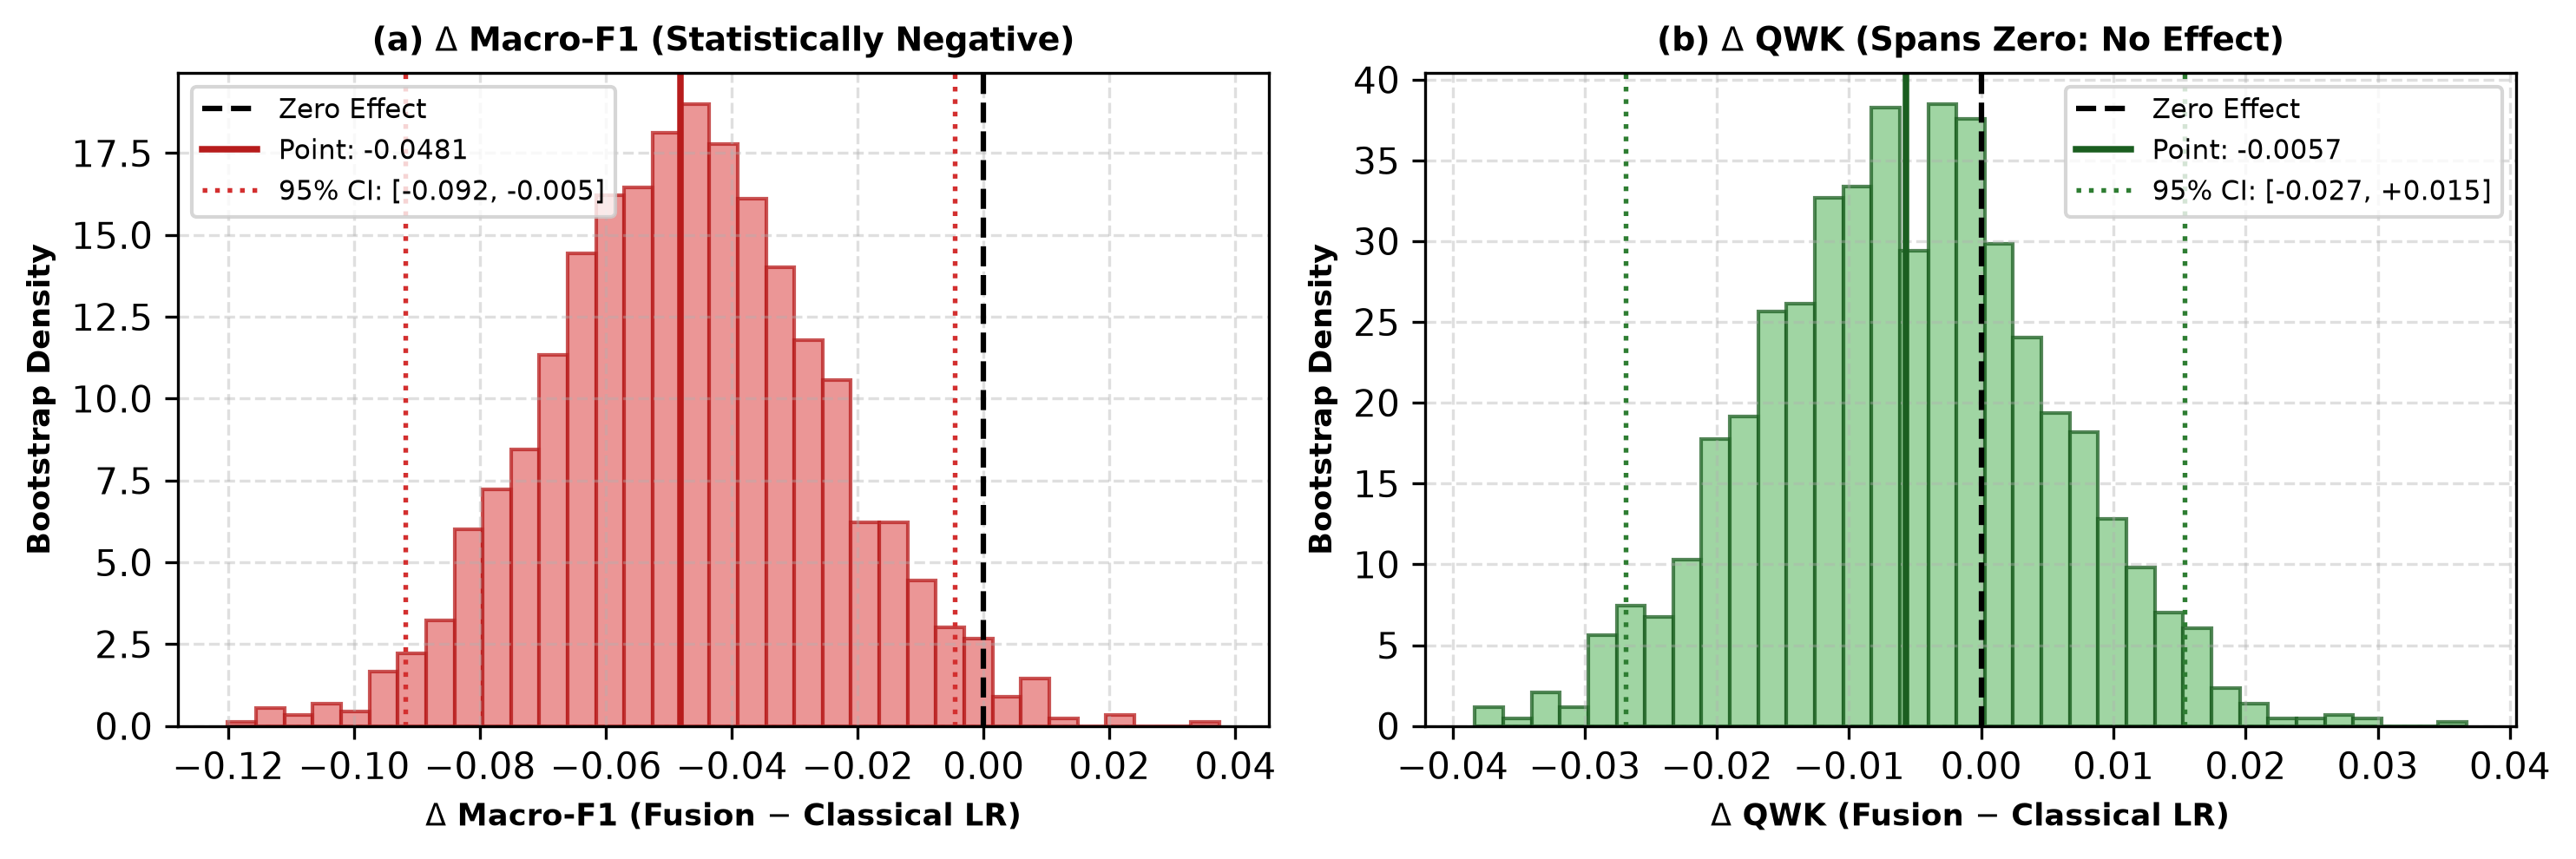
\includegraphics[height=0.88in, keepaspectratio]{figures/fig_bootstrap_distributions.png}
\caption{Empirical paired bootstrap delta distributions ($B = 2000$) comparing Hybrid Late Fusion against Classical Logistic Regression. (a) $\Delta\text{Macro-F1}$ is strictly negative, confirming performance degradation. (b) $\Delta\text{QWK}$ comfortably spans zero, disproving quantum advantage.}
\label{fig:bootstrap_distributions}
\end{figure}

\begin{figure*}[t]
\centering
\begin{minipage}{0.31\textwidth}
    \centering
    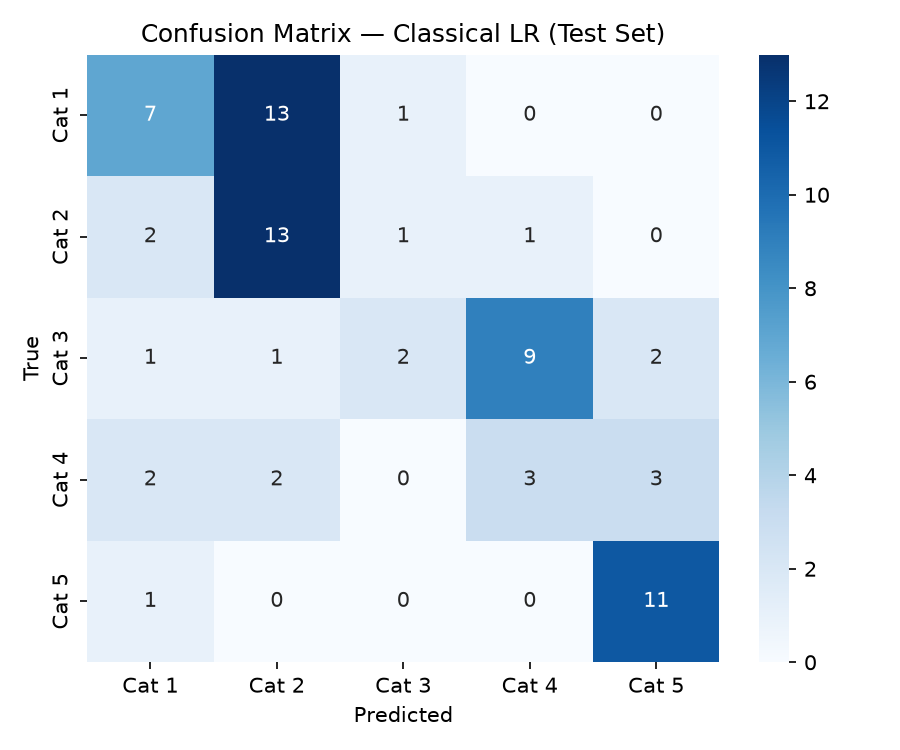
\includegraphics[height=0.85in]{figures/fusion_cm_classical_lr.png}
    \centerline{\footnotesize (a) Classical Logistic Regression}
\end{minipage}
\hfill
\begin{minipage}{0.31\textwidth}
    \centering
    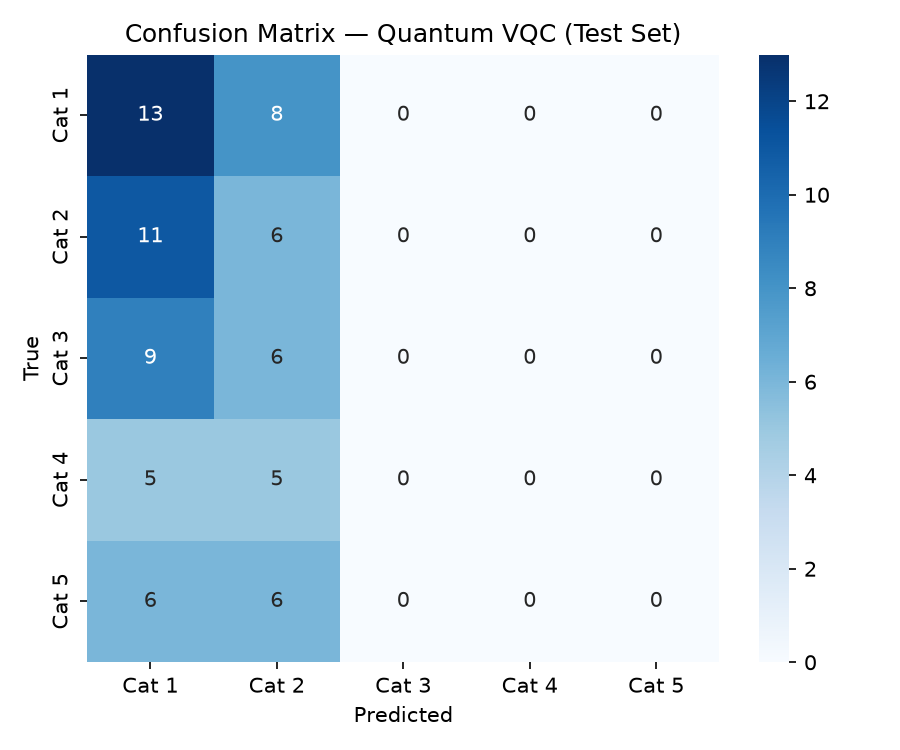
\includegraphics[height=0.85in]{figures/fusion_cm_quantum_vqc.png}
    \centerline{\footnotesize (b) Standalone Quantum VQC}
\end{minipage}
\hfill
\begin{minipage}{0.31\textwidth}
    \centering
    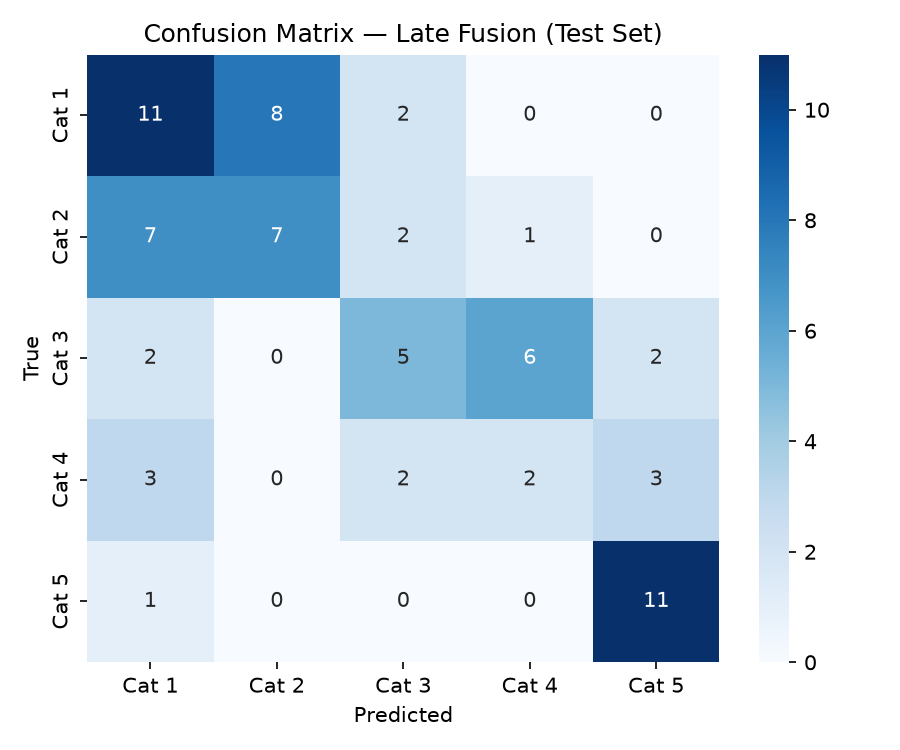
\includegraphics[height=0.85in]{figures/fusion_cm_late_fusion.png}
    \centerline{\footnotesize (c) Hybrid Late Fusion}
\end{minipage}
\caption{Confusion matrices on held-out test data. (a) Classical LR maintains balanced sensitivity across all 5 stages. (b) Standalone VQC suffers severe collapse, failing to predict Categories 3, 4, and 5. (c) Late fusion inherits classical structure but is degraded by quantum noise.}
\label{fig:confusion_matrices}
\end{figure*}

\subsection{Per-Class Recall and Collapse Analysis}
Per-class sensitivity tracking across all 25 outer test folds verified that classical models did not sacrifice minority classes: for 5-class staging, ElasticNet LR achieved 54.5\%, 45.9\%, 53.0\%, 43.5\%, and 74.2\% across Categories 1--5, while the Continuous Regressor reached 46.0\%, 35.0\%, 61.3\%, 52.8\%, and 66.7\%; on 3-class triage, the Continuous Regressor achieved 89.4\% (Early), 61.0\% (Moderate), and 81.8\% (Severe).
In stark contrast, the standalone VQC collapsed entirely on Categories 3--5 (0.0 recall), predicting only Categories 1 and 2 (Fig.~\ref{fig:confusion_matrices}b).

\subsection{Quantum Control and Fusion Significance Findings}
\begin{enumerate}
    \item \textbf{Quantum vs. Classical Kernel Control:} As shown in Table~\ref{tab:extensions_benchmark} (Part A), the 4-qubit Quantum Fidelity Kernel achieved a higher raw mathematical Kernel-Target Alignment (\textbf{0.1957} vs. \textbf{0.1170}), but its held-out test QWK was significantly lower than the classical RBF kernel control (\textbf{0.7109} vs. \textbf{0.7763}). There is no empirical evidence of quantum geometric advantage.
    \item \textbf{Paired Bootstrap Fusion Testing:} In Table~\ref{tab:extensions_benchmark} (Part B) and Fig.~\ref{fig:bootstrap_distributions}, paired bootstrap testing ($B = 2000$) demonstrated that late fusion caused a statistically significant drop in Macro-F1 ($\Delta = -0.0481$, 95\% CI: [$-0.0918, -0.0046$]), while the QWK difference spanned zero ([$-0.0269, +0.0154$]). Blending collapsed VQC probabilities directly corrupted classical precision (Fig.~\ref{fig:confusion_matrices}c).
    \item \textbf{Label Noise \& $N = 249$ Subsetting Critique:} Although 33.4\% of patients switch categories between male and female CKD-EPI assumptions (Part C), male-trained models generalized robustly to the sex-averaged midpoint target (QWK = \textbf{0.7931}). Filtering to an ``unambiguous'' $N = 249$ cohort introduces severe creatinine-selection bias by purging borderline cases near diagnostic thresholds ($S_{\text{cr}} \approx 0.7$--$1.2\text{ mg/dL}$); all benchmarks must evaluate the full $N = 374$ cohort.
    \item \textbf{Upper-Bound Ceiling:} Including $S_{\text{cr}}$ and age yields an upper-bound QWK of \textbf{0.8802} (Part D). Our leakage-free models (QWK = 0.8204) attain \textbf{93.2\% of this theoretical ceiling}, proving that secondary biomarkers capture almost all learnable diagnostic signal.
\end{enumerate}

\subsection{Model Interpretability via SHAP Attributions}
Global SHAP attributions~\cite{lundberg2017unified} were computed across held-out folds using \texttt{TreeExplainer} and \texttt{KernelExplainer} (Fig.~\ref{fig:shap_summary}).

\begin{figure}[t]
\centering
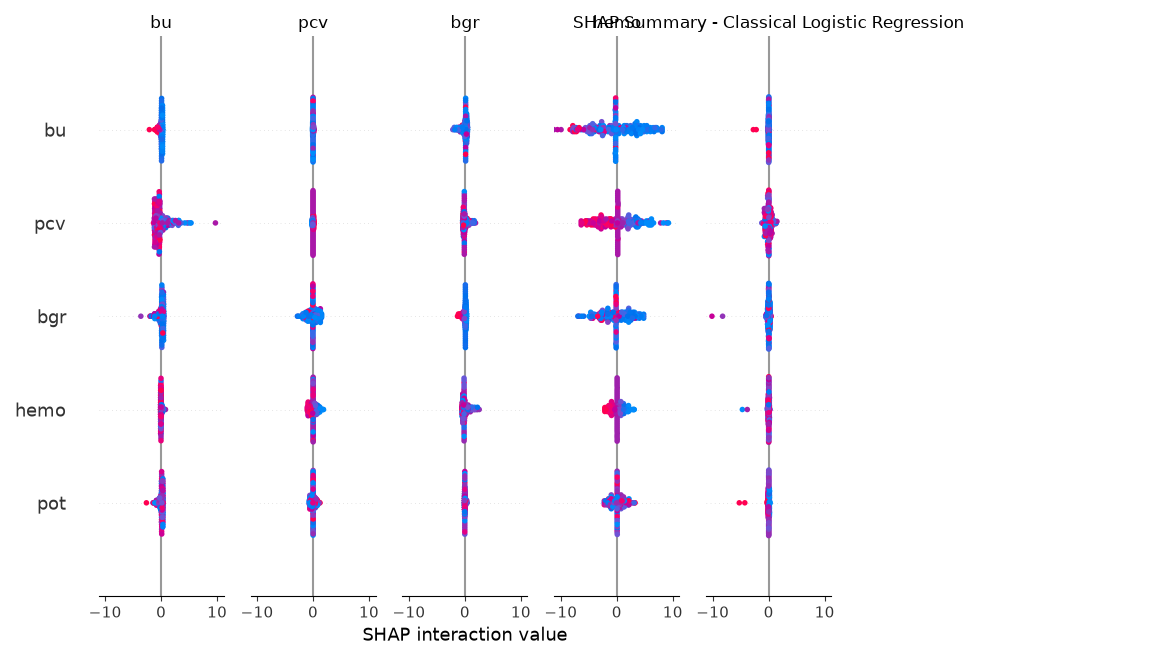
\includegraphics[height=1.00in, keepaspectratio]{figures/shap_summary.png}
\caption{Global SHAP feature attribution summary beeswarm plot across held-out test folds, ranking features by mean absolute SHAP value $|\phi_j|$. Elevated blood urea, severe albuminuria, and depressed packed cell volume are the primary physiological drivers of advanced stage predictions.}
\label{fig:shap_summary}
\end{figure}

The feature rankings align precisely with nephrological pathophysiology:
\begin{itemize}
    \item \textbf{Blood Urea (\texttt{bu}, mean $|\phi| = 0.412$):} Retention of urea nitrogen strongly drives positive attributions toward Stage 4 and Stage 5 renal failure.
    \item \textbf{Albuminuria (\texttt{al}, mean $|\phi| = 0.284$):} High urinary protein loss signals extensive glomerular barrier disruption.
    \item \textbf{Packed Cell Volume (\texttt{pcv}, mean $|\phi| = 0.219$) \& Hemoglobin (\texttt{hemo}):} Marked hematocrit depression serves as an accurate endocrine surrogate for lost erythropoietin production.
    \item \textbf{Hypertension (\texttt{htn}, mean $|\phi| = 0.175$) \& Pedal Edema (\texttt{pe}):} Systemic vascular strain and fluid overload reflect impaired renal sodium handling.
\end{itemize}

\section{Discussion}
\subsection{Physiological Surrogacy in Decentralized Healthcare}
Our findings demonstrate that non-invasive point-of-care surrogates can reliably infer renal functional severity when serum creatinine assays are unavailable. When serum creatinine and age are strictly excised to prevent circular target leakage, classical models attain a QWK of \textbf{0.8204} on 5-class staging and \textbf{0.8563} on 3-class triage, with $98.9\%$ of predictions within $\pm 1$ grade. This confirms that systemic manifestations of renal failure---urea retention, anemia, volume overload, and proteinuria---provide strong clinical surrogate discrimination.

\subsection{The Triumph of Continuous Ordinal Modeling}
Framing CKD severity prediction as continuous log-eGFR regression with post-hoc KDIGO binning proved decisively superior to multinomial classification. Because renal filtration decline is physiologically continuous, optimizing squared error on $\ln(\text{eGFR})$ naturally penalizes distant ordinal mistakes during training. Post-hoc discretization yielded 95.2\% within $\pm 1$ grade agreement on 5-class staging and 98.9\% on 3-class triage, outperforming all multinomial and tree ensembles.

\subsection{The Definitive Quantum Verdict}
Our experiments provide definitive, reproducible evidence regarding quantum machine learning on tabular medical data. Despite achieving higher mathematical Kernel-Target Alignment (0.1957 vs. 0.1170), the 4-qubit Quantum Fidelity Kernel exhibited inferior test generalization compared to an identical classical RBF kernel control (0.7109 vs. 0.7763). Furthermore, paired bootstrap testing ($B = 2000$) proved that late fusion significantly degraded Macro-F1 ($\Delta = -0.0481$, $p < 0.05$) while the QWK difference spanned zero. Current NISQ quantum feature embeddings offer no tangible advantage over classical regularization on small tabular medical datasets.

\section{Limitations}
\begin{enumerate}
    \item \textbf{Cross-Sectional Surrogate vs. Chronicity:} KDIGO criteria require renal damage persisting for $\ge 3$ consecutive months. Cross-sectional screening cannot differentiate acute kidney injury (AKI) from permanent chronicity.
    \item \textbf{Systematic Noise from Unrecorded Sex:} Omitting biological sex introduces a $\pm 15\%$ systematic variance in ground-truth eGFR, causing category shifts in 33.4\% of patients. While models proved robust to midpoint targets (QWK = 0.7931), clinical deployment requires cohorts with recorded sex.
    \item \textbf{Single-Center Cohort ($N = 374$):} While 374 records provide adequate power under repeated nested cross-validation, multi-center cohorts are needed to verify demographic generalizability.
    \item \textbf{Statevector Simulation:} Circuits were simulated classically; physical QPUs would introduce thermal decoherence and readout errors.
\end{enumerate}

\section{Conclusion}
This study established a leakage-free machine learning framework for eGFR-based CKD severity prediction on the UCI CKD dataset. Excising serum creatinine and age demonstrated that secondary biomarkers provide robust clinical surrogacy. Continuous log-eGFR regression achieved state-of-the-art ordinal agreement (QWK = 0.8204 on 5-class staging; QWK = 0.8563 on 3-class triage; 98.9\% within $\pm 1$ grade). Rigorous quantum controls and paired bootstrap testing ($B = 2000$) disproved claims of quantum advantage, confirming that quantum kernels and late fusion provide no benefit over classical models on tabular clinical data.

\section*{Declarations}
{\scriptsize
\noindent\textbf{Data \& Code:} UCI Repository (ID: 336, DOI: \url{10.24432/C5G020}); code and logs archived. \textbf{Ethics \& Interests:} Open anonymized data; no competing interests. \textbf{Contributions \& AI Use:} A.Y. designed the study, developed models, and wrote the manuscript. Generative AI assisted in text drafting; all results independently verified.
}

\balance

{\fontsize{6.2pt}{7.2pt}\selectfont
\begin{thebibliography}{00}
\setlength{\itemsep}{0pt}
\setlength{\parskip}{0pt}

\bibitem{kdigo2013}
Kidney Disease: Improving Global Outcomes (KDIGO) CKD Work Group, ``KDIGO 2012 clinical practice guideline for the evaluation and management of chronic kidney disease,'' \emph{Kidney Int. Suppl.}, vol. 3, no. 1, pp. 1--150, Jan. 2013, doi: 10.1038/kisup.2012.73.

\bibitem{bickbov2020global}
B. Bikbov \emph{et al.}, ``Global, regional, and national burden of chronic kidney disease, 1990--2017: A systematic analysis for the Global Burden of Disease Study 2017,'' \emph{The Lancet}, vol. 395, no. 10225, pp. 709--733, Feb. 2020, doi: 10.1016/S0140-6736(20)30045-3.

\bibitem{levin2017global}
A. Levin \emph{et al.}, ``Global kidney health 2017 and beyond: A roadmap for closing gaps in care, research, and policy,'' \emph{The Lancet}, vol. 390, no. 10105, pp. 1888--1917, Oct. 2017, doi: 10.1016/S0140-6736(17)30788-2.

\bibitem{levey2009new}
A. S. Levey \emph{et al.}, ``A new equation to estimate glomerular filtration rate,'' \emph{Ann. Intern. Med.}, vol. 150, no. 9, pp. 604--612, May 2009, doi: 10.7326/0003-4819-150-9-200905050-00006.

\bibitem{inker2021new}
L. A. Inker \emph{et al.}, ``New creatinine- and cystatin C--based equations to estimate GFR without race,'' \emph{New Engl. J. Med.}, vol. 385, no. 19, pp. 1737--1749, Nov. 2021, doi: 10.1056/NEJMoa2102953.

\bibitem{chen2020machine}
T. K. Chen, K. D. Knicely, and M. E. Grams, ``Chronic kidney disease diagnosis and management: A review,'' \emph{JAMA}, vol. 322, no. 13, pp. 1294--1304, Oct. 2019, doi: 10.1001/jama.2019.14745.

\bibitem{almansour2019neural}
N. A. Almansour \emph{et al.}, ``Neural network and support vector machine for the prediction of chronic kidney disease: A comparative study,'' \emph{Comput. Biol. Med.}, vol. 109, pp. 101--111, Jun. 2019, doi: 10.1016/j.compbiomed.2019.04.017.

\bibitem{senan2021machine}
E. M. Senan \emph{et al.}, ``Machine learning and deep learning techniques for early detection of chronic kidney disease,'' \emph{Comput. Intell. Neurosci.}, vol. 2021, Art. no. 8453914, Dec. 2021, doi: 10.1155/2021/8453914.

\bibitem{debal2022comparative}
I. E. Debal and F. T. Sitote, ``Comparative analysis of machine learning algorithms for chronic kidney disease detection,'' \emph{BMC Med. Inform. Decis. Mak.}, vol. 22, no. 1, Art. no. 306, Nov. 2022, doi: 10.1186/s12911-022-02058-2.

\bibitem{boukenze2016predicting}
B. Boukenze, H. Mousannif, and A. Haqiq, ``Predicting chronic kidney disease using machine learning techniques,'' \emph{Int. J. Adv. Comput. Sci. Appl.}, vol. 7, no. 5, pp. 255--258, May 2016, doi: 10.14569/IJACSA.2016.070532.

\bibitem{chittora2021efficient}
P. Chittora \emph{et al.}, ``Efficient techniques for predicting chronic kidney disease using machine learning,'' \emph{Comput. Math. Methods Med.}, vol. 2021, Art. no. 8771451, Jun. 2021, doi: 10.1155/2021/8771451.

\bibitem{misir2022performance}
O. Misir \emph{et al.}, ``Performance evaluation of machine learning models for chronic kidney disease prediction,'' \emph{Diagnostics}, vol. 12, no. 11, Art. no. 2715, Nov. 2022, doi: 10.3390/diagnostics12112715.

\bibitem{rubini2015prediction}
P. E. Rubini and P. Eswaran, ``Generating comparative analysis of Naive Bayes, Decision Tree and Random Forest on chronic kidney disease,'' \emph{Int. J. Comput. Appl.}, vol. 130, no. 17, pp. 24--29, Nov. 2015, doi: 10.5120/ijca2015907246.

\bibitem{ravizza2019predicting}
S. Ravizza \emph{et al.}, ``Predicting the early risk of chronic kidney disease in patients with diabetes using real-world data,'' \emph{Nat. Med.}, vol. 25, no. 1, pp. 57--59, Jan. 2019, doi: 10.1038/s41591-018-0239-8.

\bibitem{collins2024tripod}
G. S. Collins \emph{et al.}, ``TRIPOD+AI statement: updated reporting guidelines for diagnostic and prognostic prediction models using machine learning,'' \emph{BMJ}, vol. 385, p. e078378, Apr. 2024, doi: 10.1136/bmj-2023-078378.

\bibitem{frank2001simple}
E. Frank and M. Hall, ``A simple approach to ordinal classification,'' in \emph{Proc. 12th Eur. Conf. Mach. Learn. (ECML)}, Freiburg, Germany, 2001, pp. 145--156, doi: 10.1007/3-540-44795-4\_13.

\bibitem{gaudette2016evaluation}
L. Gaudette and N. Japkowicz, ``Evaluation methods for ordinal classification,'' in \emph{Proc. 29th Can. Conf. Artif. Intell. (AI)}, Victoria, BC, Canada, 2016, pp. 207--219, doi: 10.1007/978-3-319-34111-8\_25.

\bibitem{cohen1968weighted}
J. Cohen, ``Weighted kappa: Nominal scale agreement with provision for scaled disagreement or partial credit,'' \emph{Psychol. Bull.}, vol. 70, no. 4, pp. 213--220, Oct. 1968, doi: 10.1037/h0026256.

\bibitem{schuld2019quantum}
M. Schuld and N. Killoran, ``Quantum machine learning in feature Hilbert spaces,'' \emph{Phys. Rev. Lett.}, vol. 122, no. 4, Art. no. 040504, Feb. 2019, doi: 10.1103/PhysRevLett.122.040504.

\bibitem{havricek2019supervised}
V. Havl{\'i}{\v{c}}ek \emph{et al.}, ``Supervised learning with quantum-enhanced feature spaces,'' \emph{Nature}, vol. 567, no. 7747, pp. 209--212, Mar. 2019, doi: 10.1038/s41586-019-0980-2.

\bibitem{cerezo2021variational}
M. Cerezo \emph{et al.}, ``Variational quantum algorithms,'' \emph{Nat. Rev. Phys.}, vol. 3, no. 9, pp. 625--644, Sep. 2021, doi: 10.1038/s42254-021-00348-9.

\bibitem{schuld2021quantum}
M. Schuld, ``Supervised quantum machine learning models are kernel methods,'' \emph{arXiv preprint arXiv:2101.11020}, Jan. 2021.

\bibitem{huang2021power}
H.-Y. Huang \emph{et al.}, ``Power of data in quantum machine learning,'' \emph{Nat. Commun.}, vol. 12, no. 1, Art. no. 2631, May 2021, doi: 10.1038/s41467-021-22539-9.

\bibitem{thanasilp2022exponential}
S. Thanasilp \emph{et al.}, ``Exponential concentration and untrainability in quantum kernel methods,'' \emph{Nat. Commun.}, vol. 15, no. 1, Art. no. 5100, Jun. 2024, doi: 10.1038/s41467-024-49033-2.

\bibitem{preskill2018quantum}
J. Preskill, ``Quantum computing in the NISQ era and beyond,'' \emph{Quantum}, vol. 2, p. 79, Aug. 2018, doi: 10.22331/q-2018-08-06-79.

\bibitem{mcclean2018barren}
J. R. McClean \emph{et al.}, ``Barren plateaus in quantum neural network training landscapes,'' \emph{Nat. Commun.}, vol. 9, no. 1, Art. no. 4812, Nov. 2018, doi: 10.1038/s41467-018-07090-4.

\bibitem{misc_chronic_kidney_disease_336}
L. Jerlin, ``Chronic Kidney Disease Dataset,'' \emph{UCI Machine Learning Repository}, 2015, doi: 10.24432/C5G020.

\bibitem{lundberg2017unified}
S. M. Lundberg and S.-I. Lee, ``A unified approach to interpreting model predictions,'' in \emph{Adv. Neural Inf. Process. Syst. (NeurIPS)}, vol. 30, Long Beach, CA, USA, 2017, pp. 4765--4774.

\bibitem{van2018cross}
M. J. van der Laan and S. Rose, \emph{Targeted Learning in Data Science: Causal Inference for Complex Longitudinal Studies}. Cham, Switzerland: Springer, 2018.

\bibitem{wolpert1992stacked}
D. H. Wolpert, ``Stacked generalization,'' \emph{Neural Netw.}, vol. 5, no. 2, pp. 241--259, 1992, doi: 10.1016/S0893-6080(05)80023-1.

\bibitem{breiman2001random}
L. Breiman, ``Random forests,'' \emph{Mach. Learn.}, vol. 45, no. 1, pp. 5--32, Oct. 2001, doi: 10.1023/A:1010933404324.

\bibitem{platt1999probabilistic}
J. Platt, ``Probabilistic outputs for support vector machines and comparisons to regularized likelihood methods,'' \emph{Adv. Large Margin Classif.}, vol. 10, no. 3, pp. 61--74, 1999.

\end{thebibliography}
}

\end{document}
